% Default font is 11pt, which is pretty big, especially for internal
% talks Default aspect ratio is 4:3. "32", i.e. 3:2, is a compromise
% between 4:3 and 16:9
%
% Compromising on 3:2 is reasonable when you're going to show the talk
% on a projector and you don't know what kind of projector or screen it
% will be.
%
% 16:9 is best if others will be viewing it on their own devices,
% fullscreen.
%
% 4:3 is best if others will be viewing it on their own devices in a
% meeting where they want to also see the participants list/participant
% video/chat window.
%
% 3:2 is a good compromise when people will be viewing it on their own
% devices, but you don't know if they'll want to use part of the screen
% for something else or not.
%
% So 3:2 is the best default overall as of 2021. This may well change in
% the future.
%
\documentclass[aspectratio=32,10pt]{beamer}

% These together produce the same font as usual, but with copyable underscores
\usepackage[T1]{fontenc}

\usepackage{xspace}
\usepackage[absolute, overlay]{textpos}
\usepackage{verbatim}
\usepackage{graphicx}
\usepackage{array}

% Sets default width for includegraphics images
\setkeys{Gin}{width=\columnwidth}

\frenchspacing

\hypersetup{colorlinks}

\newcommand{\ul}{\begin{itemize}}
\newcommand{\lu}{\end{itemize}}
\newcommand{\ol}{\begin{enumerate}}
\newcommand{\lo}{\end{enumerate}}

\newcommand{\cols}{\begin{columns}}
\newcommand{\sloc}{\end{column}\end{columns}}

\newcommand{\col}{\begin{column}{0.5\textwidth}}
\newcommand{\colw}[1]{\begin{column}{#1\textwidth}}

\newcommand{\colbr}{\end{column}\begin{column}{0.5\textwidth}}
\newcommand{\colbrw}[1]{\end{column}\begin{column}{#1\textwidth}}

\newcommand{\hl}{$t_{1/2}$\xspace}

\newcommand{\is}[2]{\texorpdfstring{${}^{#1}$#2}{#2-#1}}

\newcommand{\meas}[4]{$(#1#2\mathrm{(stat)}#3\mathrm{(syst)})#4$}

\newcommand{\cn}{$^{\mathrm{[citation~needed]}}$\xspace}

\newcommand{\dedx}{$\mathrm{d}E/\mathrm{d}x$\xspace}
\newcommand{\piz}{$\pi^0$\xspace}
\newcommand{\pip}{$\pi^+$\xspace}
\newcommand{\pim}{$\pi^-$\xspace}
\newcommand{\mup}{$\mu^+$\xspace}
\newcommand{\mum}{\texorpdfstring{$\mu^-$\xspace}{mu\xspace}}

% "bold all" -- make both normal and math mode bold
\newcommand{\ba}[1]{{\boldmath \bf #1}}


\setbeamertemplate{navigation symbols}{} 
\mode<presentation>

% With minimal space usage for sections:
% default
% Boadilla
% Madrid
% Pittsburgh
% Rochester
%
% With space used at top for sections:
% AnnArbor
% Antibes
% Berlin
% CambridgeUS
% Copenhagen
% Darmstadt
% Dresden
% Frankfurt
% Ilmenau
% JuanLesPins
% Luebeck
% Montpellier
% Singapore
% Szeged
% Warsaw
%
% With space used on right or left for sections:
% Berkeley
% Goettingen
% Hannover
% Malmoe
% Marburg
% PaloAlto
%
% With space used on left for ... something:
% Bergen
\usetheme{PaloAlto}
% default
% albatross
% beaver
% beetle
% crane
% dolphin
% dove
% fly
% lily
% orchid
% rose
% seagull
% seahorse
% whale
% wolverine
\usecolortheme{default}

\setbeamersize{text margin left=2mm,text margin right=2mm} 

\author{Matthew Strait}
\institute{University of Minnesota}

%%%%%%%%%%
% Tricks %
%%%%%%%%%%

\newcommand{\beginbackup}{
   \newcounter{framenumbervorappendix}
   \setcounter{framenumbervorappendix}{\value{framenumber}}
}
\newcommand{\backupend}{
   \addtocounter{framenumbervorappendix}{-\value{framenumber}}
   \addtocounter{framenumber}{\value{framenumbervorappendix}} 
}

\newcommand{\topbit}[3]{
  \title[#3]{#1}
  \pdfinfo{
     /Author (Matthew Strait)
     /Title  (#1)
  }
  \date{#2}

  \begin{document}

  \frame{
   \maketitle
  }

}

\usepackage{tikz}

\newcommand{\hcancel}[1]{%
    \tikz[baseline=(tocancel.base)]{
        \node[inner sep=0pt,outer sep=0pt] (tocancel) {#1};
        \draw[black] (tocancel.west) -- (tocancel.east);
    }%
}%

\setbeamertemplate{footline}[frame number]


\topbit{Thoughts about gravitational wave follow-up and LIGO triggering}{15 June 2017}
       {GW, LIGO}

\section{Intro}

\frame{\frametitle{Outline}

\ul

\item Potential signals: black hole and/or neutron star mergers, supernovae, misc

\item Work so far

\item Analyzing existing data

\item Triggering on future events

\lu

}


\frame{\frametitle{Black hole/black hole mergers}

\begin{center}
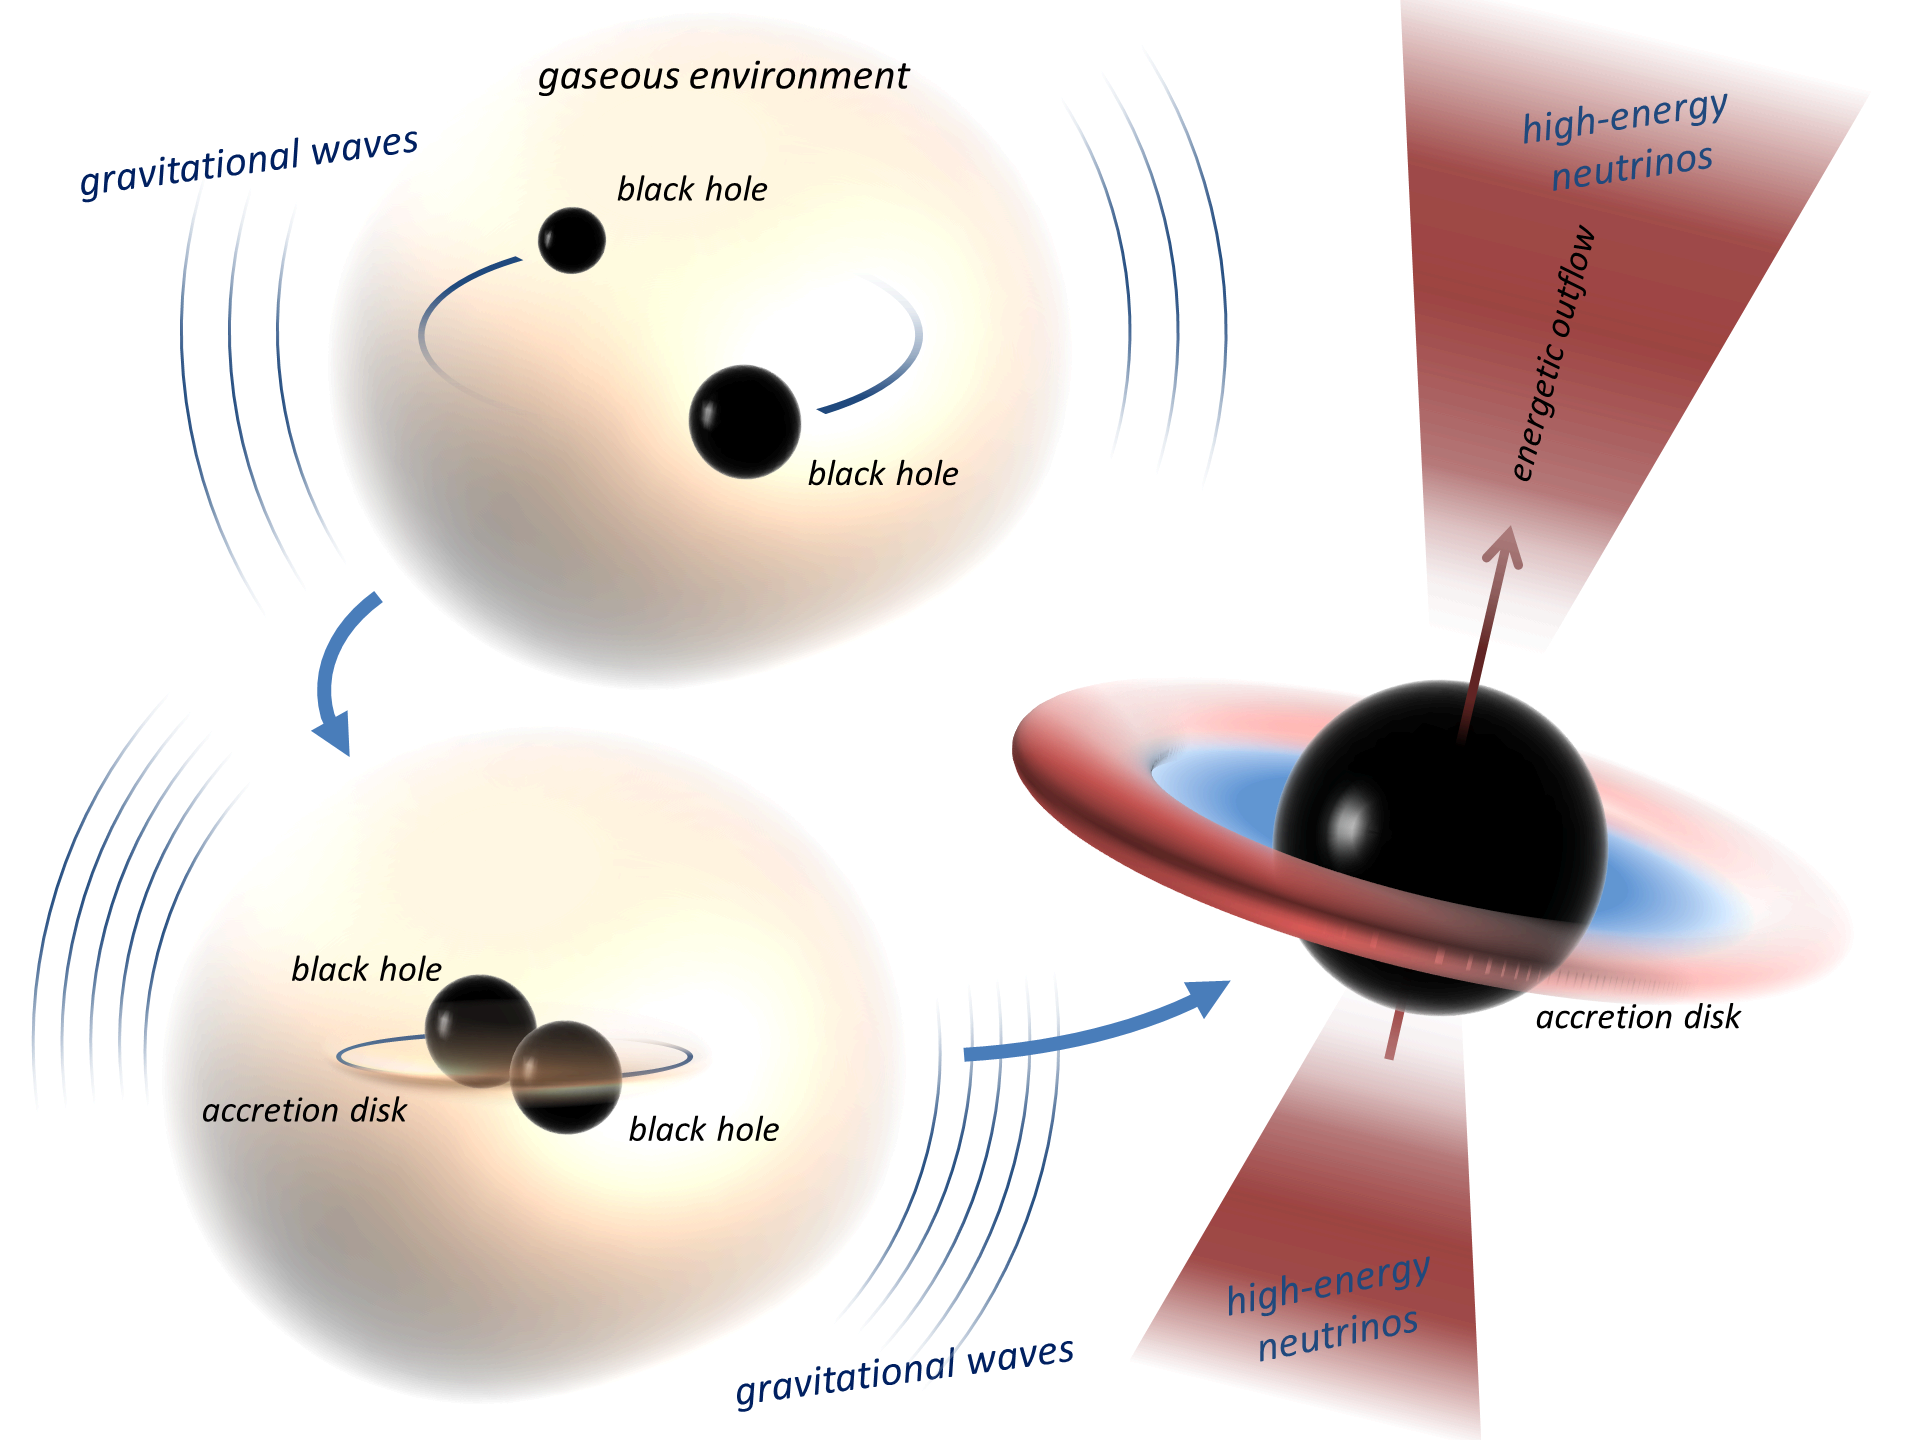
\includegraphics[width=0.5\columnwidth]{fig-bhbh-nu-64.png}
\end{center}

\ul

  \item All LIGO events so far

  \item Sensitivity to O(Gpc)

  \item If surrounded by gas, there might be a neutrino signal

  \item And also cosmics? But not necessarily pointing back to the source?

  \item IceCube and ANTARES did a neutrino search: null

  \item Neutron star/black hole mergers are similar, I think

\lu

}

\frame{\frametitle{Neutron star/neutron star mergers}

\begin{center}
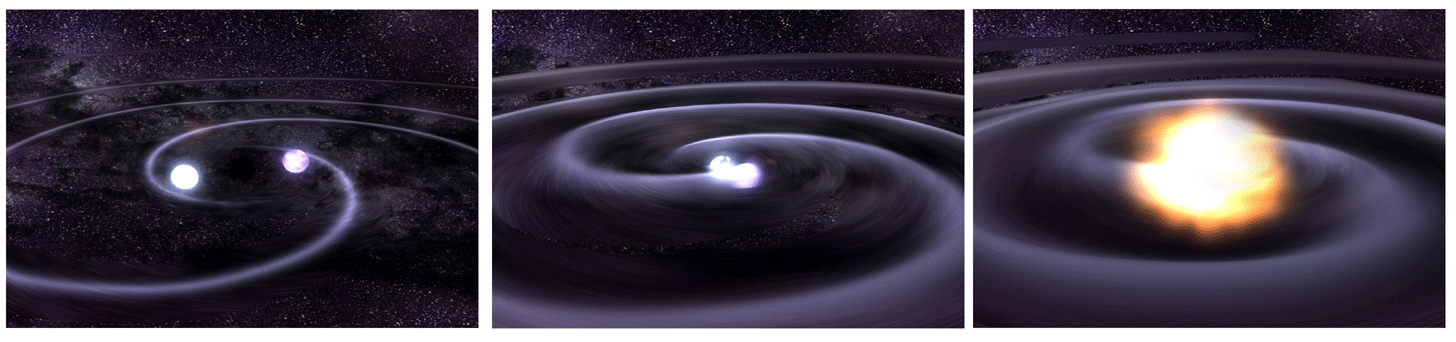
\includegraphics[width=\columnwidth]{fig-nsns-merger.jpg}
\end{center}

\ul

\item Clearly are going to make some thermal and nucleosynthesis
neutrinos: \href{https://arxiv.org/abs/1510.06398}{arXiv:1510.06398}

\item Higher energy neutrinos from the inspiral? 
\href{http://www.sciencedirect.com/science/article/pii/S2214404816300118}{Example paper}

\item Galactic rate estimated at 0.01/century, so if no higher energy signal, no
real hope\dots

\item LIGO reach is about half that for black
hole mergers (i.e. quite distant)

\lu

}

\frame{\frametitle{Supernovae}

\begin{center}
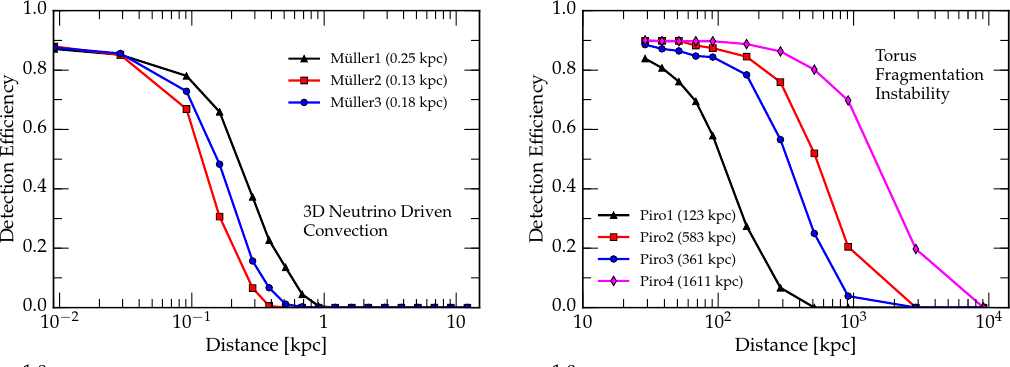
\includegraphics[width=0.56\columnwidth]{fig-ligo-supernova-sensitivity.png}
\end{center}

\ul

  \item Large neutrino signal if it is in the galaxy

  \item LIGO reach very poorly understood (\href{https://arxiv.org/abs/1605.01785}{arXiv:1605.01785})
  
  \item Models range from 130\,pc (10\% of seeing Antares or
  Betelgeuse) to 740\,kpc (covers our galaxy and P=50\% for Andromeda)

  \item The paper is rather guarded, but lower end sounds more likely

  \item Anyway, it's an independent SNEWS-like warning, maybe

\lu

}

\frame{\frametitle{Misc unknown}

\cols

\colw{0.6}

\ul

  \item LIGO does a generic ``burst'' search

  \item ``Every time humans have looked at the universe with a new set of `eyes' [\dots] they have found things that were unexpected and revolutionized our understanding of the universe''
  
  \item ``Therefore, in burst gravitational waves we are expecting the unexpected''

  \item Could find something:
  \ul
    \item Relatively mundane: whatever makes gamma ray bursts, stellar-mass star mergers
    \item Exotic, but described: oscillating cosmic strings (\href{https://arxiv.org/abs/0904.4718}{arXiv:0904.4718}), domain walls
    \item Something totally unanticipated
  \lu

\lu

\colbrw{0.4}

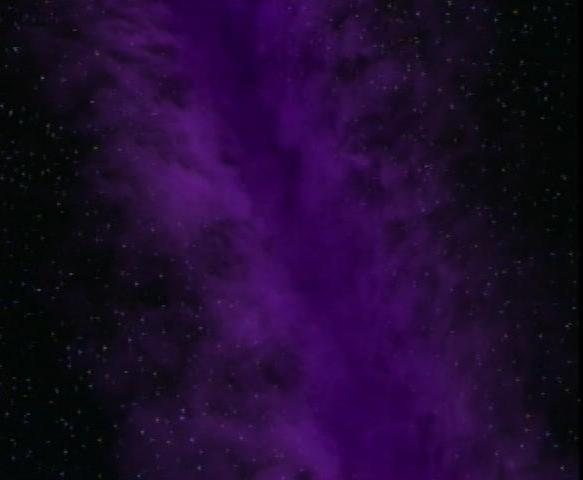
\includegraphics[width=\columnwidth]{fig-star-trek-cosmic-string.jpg}

\sloc

}

\section{So far}

\frame{\frametitle{So far}

\ul

\item Alec took a look our data coincident with the first
LIGO event in \href{http://nova-docdb.fnal.gov:8080/cgi-bin/ShowDocument?docid=14351}{doc-14351}

\item Was on 2015-09-14, during shutdown.


  \ul

    \item FD was up, but ``ratty'', in Alec's words.

    \item ND was running smoothly.

  \lu


\item 2nd good LIGO event on 2015-12-26 3:38:53 UTC:

  \ul
  \item Both detectors running smoothly.
  \lu

\item 3rd good LIGO event on 2017-01-04 10:11:58.6 UTC

  \ul
  \item Both detectors running smoothly.
  \lu

\item Marginal LIGO event on 2016-10-12 9:54:43 UTC

  \ul
  \item FD down ``Error in DataLogger''. 
  \item ND ok.
  \lu

\lu

}

\section{Analysis}

\frame{\frametitle{Analysis}

Signals:

\ul

\item Low-to-medium energy muons: FD samples lower energy, ND higher energy

\item High-energy cosmics: Look for large showers at the FD

\item MeV neutrinos: supernova or supernova-like signal

\item GeV neutrinos: upward-going muons or any burst of contained events

\lu

Do we have unique capabilities?

\ul

\item Lower energy muons?  Maybe.

\item Higher energy muons? Less likely.  Cosmic ray arrays are better
suited to this.

\item MeV neutrinos? Yes.  We are a large carbon detector and provide 
flavor information when combined with detectors of other compositions.

\item GeV neutrinos: Probably.  Our mass is comparable to Super-K.

\item Higher energy neutrinos: No, IceCube is much better

\lu

}

\section{Triggering}

\frame{\frametitle{Triggering}

\ul

\item Our only data for the LIGO events so far is sampled at 0.55\% by the 10\,Hz 
trigger, plus O(0.1\%) by other triggers

\item Would be lovely to have all the data instead

\item LIGO --- actually LIGO/VIRGO --- sends out prompt alerts to groups that
have signed \href{https://dcc.ligo.org/LIGO-M1300550/public}{an MOU} with them

\lu

}

\frame{\frametitle{Triggering details}

\ul

\item Latency: ``about 1 minute'' --- this is for the ``preliminary alert''
with no directionality, no human check: that fine for us

\item Higher confidence alerts follow in a ``few minutes'' and ``hours or
more'', but we don't need high confidence to trigger as long as the rate is
manageable.

\item Which it is: their target is around 1 per month

\item What length would we read out?

\ul

  \item For mergers, a potential neutrino burst is probably O(1\,s) (?)
  \item For supernovae, we have an answer: 45\,s
  \item For exotic/unanticipated events, obviously can't say
\lu

\item The alert will not tell us which one it is $\rightarrow$ 45\,s

\item Besides being a GW alert, it would be operationally nice to have a
SNEWS-like trigger that actually triggers sometimes (and not just 
at 8:30am)

\lu

}

\section{Conclusions}

\frame{\frametitle{Conclusions}

\ul

\item Could be some interesting physics in gravitational wave coincidences

\item We should analyze the data already taken and write a paper

\item We should consider triggering on LIGO alerts

\lu

}

\beginbackup

\frame{\frametitle{Backups}}

\backupend
%%%%%%%%%%%%%%%%%%%%%%%%%%%%%%%%%%%%%%%%%%%%%%%%%%%%%%%%%%%%%%%%%%%%%%%%
\end{document}
